% Predlozak za pisanje diplomskog rada na PMF-MO
% Opcenita uputstva za LaTeX se mogu npr. naci na 
% http://web.math.hr/nastava/rp3, http://web.math.hr/nastava/s4-prof/latex.pdf
% NE PREPORUCA se "Ne baš tako kratak uvod u TEX", buduci se radi o vrlo starom prirucniku
% koji nije pogodan za moderne verzije LaTEXa.
% Originalna verzija "The not so short..." na http://tobi.oetiker.ch/lshort/lshort.pdf 
% je obnovljena i daje bolji uvid u moderne verzije LaTeXa

% Stil je optimiziran za kreiranje pdf dokumenta (npr. pomocu pdflatex-a, XeLaTeX-a)

\documentclass[a4paper,twoside,12pt]{memoir} % jednostrano: promijeniti twoside u oneside

% Paket inputenc omogucava direktno unosenje hrvatskih dijakritickih znakova 
% opcija utf8 za unicode (unix, linux, mac)
% opcija cp1250 za windowse
\usepackage[utf8]{inputenc}  % ukoliko se koristi XeLaTeX onda je \usepackage{xunicode}\usepackage{xltxtra}

% Stil za diplomski, unutra je ukljucena podrska za hrvatski jezik
\usepackage{diplomski}
% bibliografija na hrvatskom
\usepackage[languagenames,fixlanguage,croatian]{babelbib} % zahtijeva datoteku croatian.bdf
% hiperlinkovi 
\usepackage[pdftex]{hyperref} % ukoliko se koristi XeLaTeX onda je \usepackage[xetex]{hyperref}

% Odabir familije fontova:
% koristenjem XeLaTeX-a mogu se koristiti svi fontovi instalirani na racunalu, npr
% \defaultfontfeatures{Mapping=tex-text}
% \setmainfont[Ligatures={Common}]{Hoefler Text}
% ili
% \newcommand{\nas}[1]{\fontspec{Adobe Garamond Pro}\fontsize{24pt}{24pt}\color{Chocolate}\selectfont #1}
% i onda \nas{Naslov ...}
\usepackage{txfonts} % times new roman 

% Paket graphicx sluzi za manipuliranje grafikom 
\usepackage[pdftex]{graphicx} % ukoliko se koristi XeLaTeX onda je \usepackage[xetex]{graphicx}
% Paket amsmath je vec ukljucen
% Dodatno definirane matematicke okoline:
% teorem (okolina: thm), lema (okolina: lem), korolar (okolina: cor),
% propozicija (okolina: prop), definicija (okolina: defn), napomena (okolina: rem),
% slutnja (okolina: conj), primjer (okolina: exa), dokaz (okolina: proof)
% Definirane su naredbe za ispisivanje skupova N, Z, Q, R i C
% Definirane su naredbe za funkcije koje se u hrvatskoj notaciji oznacavaju drukcije 
% nego u americkoj: tg, ctg, ... (\tgh za tangens hiperbolni)
% Takodjer su definirane naredbe za Ker i Im (da bi se razlikovala od naredbe za imaginarni dio kompleksnog
% broja, naredba se zove \slika).

\pagestyle{headings}
% uz paket fancyhdr mogu se lako kreirati fancy zaglavlja i podnozja

% Podaci koje treba unijeti
\title{Naslov}
\author{Ime Prezime}
\advisor{Ime Profesora}  % obavezno s titulom (prof. dr. sc ili doc. dr. sc.)
\date{Godina}  % oblika mjesec, godina

% Moguce je unijeti i posvetu
% Ukoliko nema posvete, dovoljno je iskomentirati/izbrisati sljedeci redak 
\dedication{Samom sebi}

\begin{document}

% Naredna frontmatter generira naslovnu stranicu, stranicu za potpise povjerenstva, eventualnu posvetu i sadrzaj
% Moze se iskomentirati ukoliko nije u pitanju konacna verzija
\frontmatter

% Tekst diplomskog ...

% Diplomski rad treba poceti s uvodnim poglavljem  
\begin{intro}
...
\end{intro}

\chapter[Naslov poglavlja u sadržaju][Kratki naslov poglavlja]{Naslov poglavlja}	
% ukoliko naslov nije jako dugacak dovoljno je samo \chapter{Naslov poglavlja} 

\section[Naslov sekcije u sadržaju][Kratki naslov sekcije]{Naslov sekcije}
\subsection{Naslov podsekcije}
\begin{thm}
Iskaz teorema u kojem se javljaju skupovi  $\N$, $\Z$, $\Q$, $\R$ i $\C$.
\end{thm}
\begin{conj}
Iskaz slutnje u kojoj se javljaju funkcije $\tg$, $\tgh$ i $\sh$.
\end{conj}
\begin{cor}
Iskaz posljedice u kojoj se javljaju skupovi $\Ker T$ i $\slika T$..
\end{cor}
\begin{proof}
Dokaz posljedice se nalazi u \cite{kljuc}. Pogledajte i \cite{kurepa1956convex}, \cite{kurepa1981funkcionalna} te \cite{Dutkay:2009}.
\end{proof}
jsfdsqF
SG
SFG
FSG
DF
GS
FG
SFG
SFG

SFG

SG
SDFG
SF
GS

DG
 SD
S


SD
 

DFGSDFG


SDGSDF


SDGSDGF


SDGFSFDG


SDGSDG  sdfsfg f fdh fgj gh jgjk jkj k yk k klk l fs fd gsdfg dfh dfghj fj ghjk gjk jlk sdf 
$x_1+x_2+x_3+x_4=12$ $x_1+x_2+x_3+x_4=12$
 $x_1+x_2+x_3+x_4=12$ $x_1+x_2+x_3+x_4=12$ $x_1+x_2+x_3+x_4=12$ $x_1+x_2+x_3+x_4=12$
 $x_1+x_2+x_3+x_4=12$ $x_1+x_2+x_3+x_4=12$ $x_1+x_2+x_3+x_4=12$
$x_1+x_2+x_3+x_4=12$ 
SDGSG sdfsfg f fdh fgj gh jgjk jkj k yk k klk l fs fd gsdfg dfh dfghj fj ghjk gjk jlk sdf sfdh j fj tuk ugad h j yrtu iru i
\[ z \left( 1 \ +\ \sqrt{\omega_{i+1} + \zeta -\frac{x+1}{\Theta +1} y + 1}
\ \right) =  1 \]

GSDFGSDFG



\begin{equation}
\label{eq:jed1}
	1+1=2
\end{equation}

SDG
SDFGS

SDFGSFG


SFGSFG


SDFGSFG


SDGSFG

\label{stranica}
Na stranici \pageref{stranica} se nalaza slika u \textbf{png} formatu.
% slike smiju biti u svim formatima koje podrzava pdf (pdf, jpg, png)
\begin{figure}[h!t]
\begin{center}

\includegraphics[scale=0.5]{mosaic-from-pompeii.png}
\caption{Prva slika}
\end{center}
\end{figure}

Na slici \ref{fig:3d} se nalazi 3D graf neke funkcije. 

\begin{figure}[h!t]
\centering 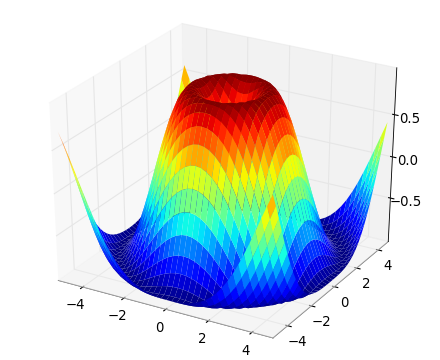
\includegraphics{surface3d.png}
\caption{Druga slika}
\label{fig:3d}
\end{figure}

kao i jedna vrlo komplicirana formula koja slijedi iz \eqref{eq:jed1}
\[ \sum_{i=1}^{\infty}A_{x_1}\times A_{{\alpha}_2}\oslash\iint_{\Omega}x^2\ddagger\limsup_{n\in\N}\frac{\alpha+\theta+\gamma}{n^{\omega}}\;\;\text{je u stvari}\;\;\biguplus_{r\in\Q}\overline{\Xi_i \mathop\Theta_{\substack{j\in\C \\ j\ni i\Q}} \Upsilon^{k^j} \underset{\ast}{\Psi} \hslash\vert_{\{\alpha\}}}.\]

% Na kraju diplomkog rada stavlja se  bibliografija
% Najprije definiramo nacin prikazivanja bibliografije, u ovom slucaju verzija amsplain stila
\bibliographystyle{babamspl} % babamspl ili babplain

% U datoteku diplomski.bib se stavljaju bibliografske reference
% Bibliografske reference u bib formatu se mogu dobiti iz MathSciNet baze, Google Scholara, ArXiva, ...
\bibliography{diplomski}

\pagestyle{empty} % ne zelimo brojanje sljedecih stranica

% I na koncu idu sazeci na hrvatskom i engleskom

\begin{sazetak}
Ukratko ...
\end{sazetak}

\begin{summary}
In this ...
\end{summary}

% te zivotopis

\begin{cv}
Dana ...
\end{cv}

\end{document}